\documentclass[11pt,a4paper]{article}

\usepackage[margin=1in]{geometry}
\usepackage[T1]{fontenc}
\usepackage[utf8]{inputenc}
\usepackage{lmodern}
\usepackage{microtype}
\usepackage{graphicx}
\usepackage{booktabs}
\usepackage{longtable}
\usepackage{array}
\usepackage{enumitem}
\usepackage{xcolor}
\usepackage{hyperref}
\usepackage{amsmath}
\usepackage{amssymb}
\usepackage{fancyhdr}
\usepackage{caption}
\usepackage{listings}

\graphicspath{{../assets/}{../public/assets/}{assets/}{public/assets/}}

\definecolor{AstroBlue}{HTML}{38BDF8}
\definecolor{AstroViolet}{HTML}{A78BFA}
\definecolor{AstroDark}{HTML}{020617}
\definecolor{AstroGray}{HTML}{475569}

\hypersetup{
  colorlinks=true,
  linkcolor=AstroViolet,
  urlcolor=AstroBlue,
  citecolor=AstroViolet,
  pdftitle={AstroBis Project Report},
  pdfauthor={Biswajit Jana}
}

\lstdefinestyle{astrobis}{
  basicstyle=\ttfamily\small,
  breaklines=true,
  frame=single,
  rulecolor=\color{AstroGray},
  backgroundcolor=\color{black!3}
}

\pagestyle{fancy}
\fancyhf{}
\lhead{AstroBis Project Report}
\rhead{Biswajit Jana}
\cfoot{\thepage}

\title{
  \vspace{-1.2cm}
  \textbf{\Huge AstroBis}\\[0.35em]
  \Large A Browser-Based Scientific Astronomy and Earth Operations Platform\\[0.7em]
  \normalsize Project Report
}
\author{
  \textbf{Biswajit Jana}\\
  Independent Researcher -- Astrophysics, Instrumentation and Scientific Computing\\
  MSc Astrophysics (Advanced Research), University of Hertfordshire\\
  \href{https://biswajit1999.github.io/Biswajit_Jana.github.io/}{Academic Portfolio}
}
\date{Version 1.2.0 -- EarthOps Storm Watch Release\\August 2026}

\begin{document}
\maketitle

\begin{figure}[h]
  \centering
  \IfFileExists{../assets/astrobis-banner.png}{
    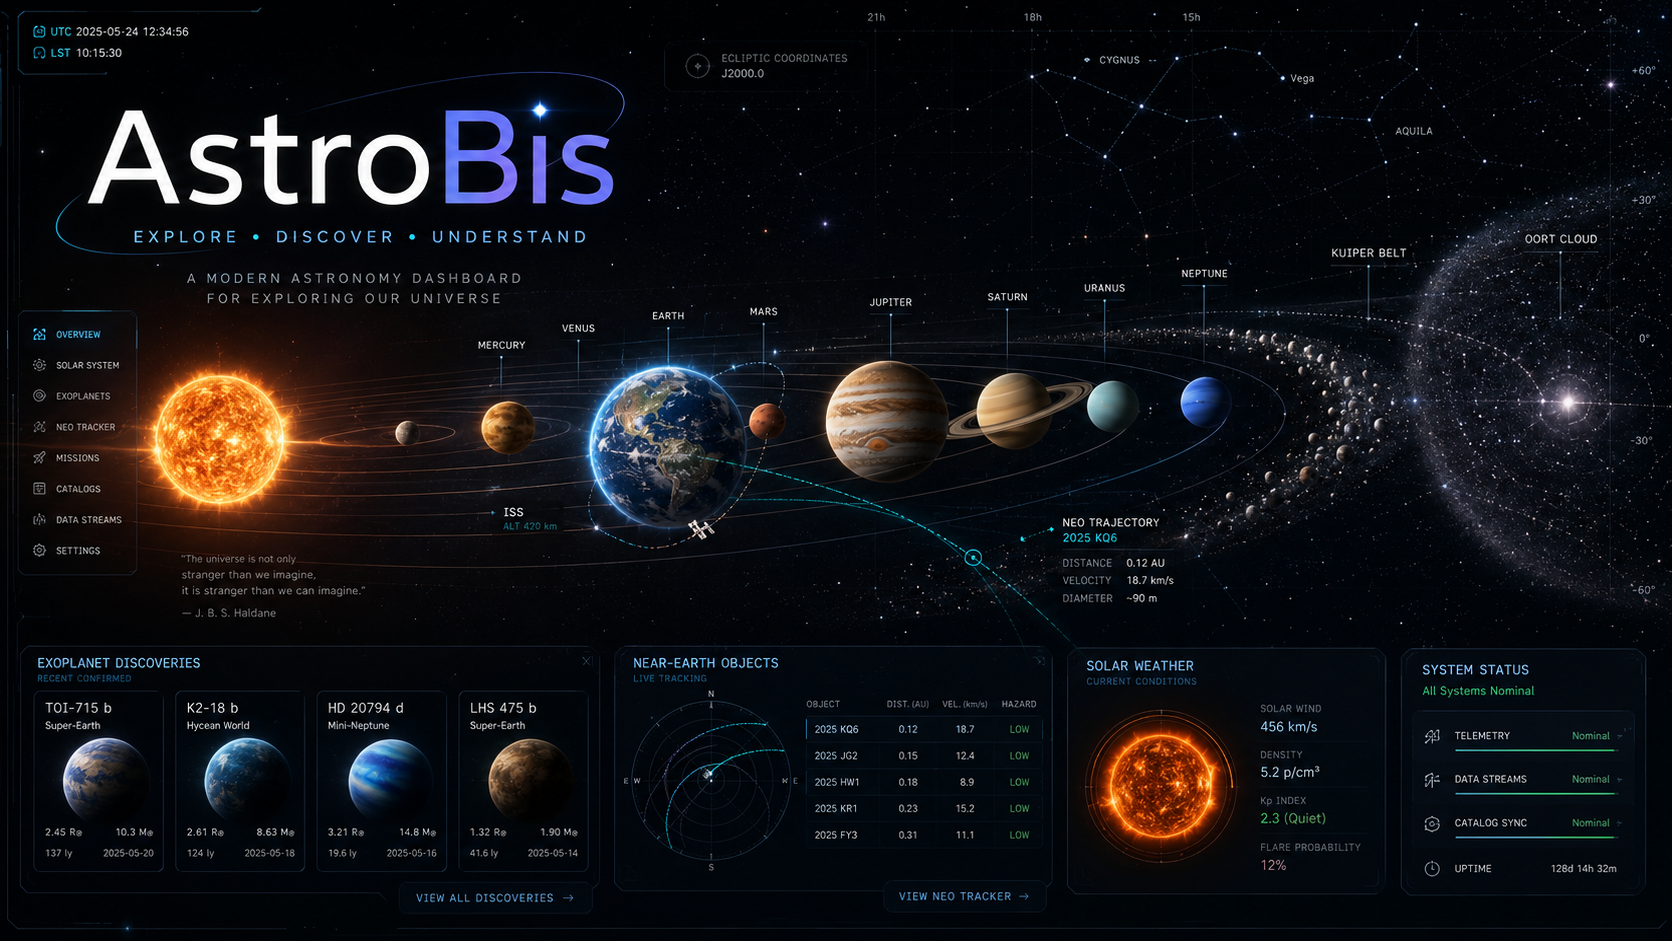
\includegraphics[width=\textwidth]{../assets/astrobis-banner.png}
  }{
    \IfFileExists{assets/astrobis-banner.png}{
      
\includegraphics[width=\textwidth]{assets/astrobis-banner.png}
    }{}
  }
  \caption{AstroBis dashboard banner: a visual summary of the Solar System, Earth operations, near-Earth objects, exoplanet discovery context, and scientific data-console design.}
  \label{fig:banner}
\end{figure}

\begin{abstract}
AstroBis is an independently developed browser-based astronomy and Earth operations platform. It combines interactive Solar System scale exploration, a Mars 3D terrain atlas, EarthOps world mapping, exoplanet catalogue analytics, International Space Station tracking, near-Earth object monitoring, interstellar visitor records, a stellar atlas, NASA astronomy content, and data-quality auditing in a single static web application. The project is designed for scientific communication: it emphasizes public-data provenance, interactive visualisation, interpretive limits, and transparent separation between measured catalogue values, derived quantities, and illustrative rendering.
\end{abstract}

\tableofcontents
\newpage

\section{Project Overview}

AstroBis was created as a public-facing scientific visualisation ecosystem for astronomy, spaceflight, and Earth-facing space infrastructure. The live website is available at:

\begin{center}
\url{https://biswajit1999.github.io/AstroBis/}
\end{center}

The primary aim is to make diverse public datasets more accessible through a coherent browser interface. AstroBis is not intended to replace specialist services such as NASA Horizons, professional flight-dynamics software, full planetarium systems, or peer-reviewed catalogue analysis pipelines. Instead, it offers an integrated scientific dashboard where a visitor can inspect scale, motion, catalogue values, uncertainty labels, and public source links.

\subsection{Design Principles}

The project follows four design principles:

\begin{enumerate}[leftmargin=*]
  \item \textbf{Scientific traceability.} The interface identifies public data sources and distinguishes archive values from interpretive visual layers.
  \item \textbf{Interactive scale.} Complex astronomical scales are compressed into navigable 3D and 2D scenes while retaining physical units such as astronomical units, light-time, kilometres, and parsecs.
  \item \textbf{Static deployment reliability.} Data are stored as build-time JSON snapshots so the public site remains usable even when a third-party feed fails.
  \item \textbf{Readable limitations.} Derived rankings, rendered exoplanets, Oort Cloud points, disaster markers, and hazard-style labels are treated as visual and educational proxies, not official scientific determinations.
\end{enumerate}

\section{Website Structure}

AstroBis currently contains the modules listed in Table~\ref{tab:modules}. Each module is implemented as an Astro page with React and Three.js components where needed.

\begin{longtable}{p{0.24\textwidth}p{0.67\textwidth}}
\caption{AstroBis module overview.}
\label{tab:modules}\\
\toprule
\textbf{Module} & \textbf{Purpose}\\
\midrule
\endfirsthead
\toprule
\textbf{Module} & \textbf{Purpose}\\
\midrule
\endhead
Home & Entry point summarising project scope, major modules, live links, author context, and headline data counts.\\
Solar System Atlas & Interactive Sun, planets, dwarf planets, asteroid belt, Kuiper belt, heliopause, and Oort Cloud scale visualisation.\\
Mars Map & Real-texture Mars globe with NASA PDS MOLA-derived terrain, named areographic features, landing sites, coordinate picking, and moon context.\\
Exoplanets & NASA Exoplanet Archive snapshot exploration with filters, plots, discovery-method summaries, host-star context, and archive links.\\
ISS Tracker & CelesTrak GP/TLE-based ISS propagation with SGP4, 3D Earth, ground track, altitude, velocity, visibility context, and TLE age.\\
World Map & EarthOps console combining satellites, debris, launches, Earth hazards, Storm Watch, spaceflight news, public media, and location-aware mapping.\\
Small Bodies & Near-Earth close approaches through 2050, JPL small-body information, risk-style filtering, and interstellar visitor records.\\
Star Atlas & Three-dimensional bright-star orientation scene using distance shells, spectral classes, constellation guides, and physical proxies.\\
Data Quality & Snapshot audit page showing source freshness, row counts, field coverage, and data-provenance checks.\\
\bottomrule
\end{longtable}

\section{System Architecture}

AstroBis is a static web application built using Astro, React, and Three.js. The application is deployed through GitHub Pages and GitHub Actions. A snapshot-first data pipeline is used to keep the website stable.

\subsection{Technology Stack}

\begin{table}[h]
\centering
\caption{Core technology layers.}
\begin{tabular}{ll}
\toprule
\textbf{Layer} & \textbf{Technology}\\
\midrule
Site framework & Astro 4\\
Interactive UI & React 18\\
3D rendering & Three.js, @react-three/fiber, @react-three/drei\\
Post-processing & @react-three/postprocessing, postprocessing\\
Orbit propagation & satellite.js for SGP4 use cases\\
Interface icons & lucide-react\\
Styling & CSS, Tailwind configuration, responsive mobile stylesheet\\
Data pipeline & Node.js build script writing JSON snapshots\\
Deployment & GitHub Pages and GitHub Actions\\
\bottomrule
\end{tabular}
\end{table}

\subsection{Snapshot-First Data Flow}

The data pipeline is implemented in \texttt{scripts/fetch-space-data.mjs}. During a build, the script fetches public data, normalizes it into compact JSON, and writes same-origin snapshots into \texttt{public/data/}. The deployed app then loads those JSON files without requiring private server-side infrastructure.

\begin{lstlisting}[style=astrobis,caption={Simplified build-time data flow.}]
public APIs and public archives
  -> fetch-space-data.mjs
  -> normalized JSON snapshots
  -> Astro static build
  -> GitHub Pages deployment
  -> browser-side interactive modules
\end{lstlisting}

This design has two advantages. First, the live website remains functional even when a public service is temporarily unavailable. Second, each release can be connected to a clear snapshot date, source list, and row count. Browser-side refresh is used only when public CORS policy permits it.

\section{Solar System Atlas}

The Solar System Atlas visualises the system from the Sun and inner planets to the Kuiper Belt, heliopause, and Oort Cloud. A single linear scale cannot show both Earth's orbit and a distant Oort Cloud boundary. The ratio between 1 AU and 100,000 AU is:

\begin{equation}
\frac{100000}{1}=10^5.
\end{equation}

Therefore AstroBis uses compressed visual scales and selectable view modes. The atlas includes:

\begin{itemize}[leftmargin=*]
  \item eight planets and selected dwarf planets;
  \item major distance regions such as the asteroid belt, Kuiper Belt, scattered disc, heliopause, Hills Cloud, and outer Oort Cloud;
  \item AU ruler and light-time references;
  \item planet information panels including physical constants and known moons;
  \item labelled, compressed orbit paths and scale presets.
\end{itemize}

The Oort Cloud is visualised as a faint sparse spherical reservoir. This is an interpretive model: the Oort Cloud has not been directly imaged as a resolved shell. The purpose is to communicate its scale and expected comet-reservoir geometry relative to the planetary system.

\section{Mars 3D Map}

The Mars Map page is a dedicated areography console. It combines a global Mars texture, a NASA PDS Mars Global Surveyor MOLA topography layer, a hillshade layer, named feature markers, landing-site chronology, and simplified moon context.

\subsection{Mars Terrain}

The Mars terrain layer uses a same-origin WebGL heightmap derived from the MOLA MEGDR median-topography product. The heightmap is resampled for browser performance and vertically exaggerated so large-scale structures such as Olympus Mons, Valles Marineris, Hellas Planitia, and Tharsis remain visible at whole-planet scale. This is a scientific atlas layer, not a rover-scale GIS terrain engine.

\subsection{Coordinate Picking}

When the user selects a point on the Mars texture, texture coordinates $(u,v)$ are converted into latitude and longitude:

\begin{align}
\phi_{\mathrm{lat}} &= (0.5-v)\times 180^\circ,\\
\lambda_{\mathrm{lon}} &= u\times 360^\circ - 180^\circ.
\end{align}

Feature coordinates are approximate center points intended for visual navigation.

\section{EarthOps World Map}

The EarthOps World Map is a space-first operations console. It intentionally does not attempt to reproduce general news-monitoring or political OSINT maps. Its unique role is to combine space infrastructure, public Earth hazards, launches, weather context, and spaceflight news around a realistic Earth model.

\subsection{EarthOps Layers}

The page currently includes:

\begin{itemize}[leftmargin=*]
  \item 3D Earth with Blue Marble texture, city lights, clouds, atmospheric rim, stars, and terminator context;
  \item CelesTrak satellite groups, selected debris populations, stations, recent objects, and orbital-shell views;
  \item Launch Library upcoming launches and mapped launch-site coordinates;
  \item NASA EONET natural events;
  \item USGS earthquake events;
  \item GDACS disaster alerts;
  \item Storm Watch using public weather-radar metadata and storm-related event records;
  \item spaceflight news and public media source cards;
  \item optional browser geolocation for marking the visitor's approximate position.
\end{itemize}

\subsection{Storm Watch Release}

Version 1.2.0 added Storm Watch. This release introduced:

\begin{itemize}[leftmargin=*]
  \item public radar-frame metadata from RainViewer;
  \item storm, cyclone, and flood advisory records derived from public NASA EONET and GDACS records;
  \item animated storm bands on the 3D globe;
  \item selectable storm markers in the 3D globe, 2D operations map, mini map, and bottom timeline;
  \item source-health information for weather/radar layers.
\end{itemize}

The release snapshot contained five storm advisories and twelve public radar frames at build time. These values will change as the build pipeline refreshes public feeds. Public weather products can be delayed, so AstroBis labels this layer as public near-real-time situational context, not as an official forecast.

\subsection{Earth Surface Geometry}

Surface markers are placed on a visual sphere through the standard spherical coordinate conversion:

\begin{align}
x &= R\cos\phi\cos\lambda,\\
y &= R\sin\phi,\\
z &= -R\cos\phi\sin\lambda,
\end{align}

where $\phi$ is latitude, $\lambda$ is longitude, and $R$ is the visual Earth radius. This is suitable for visual marker placement. It is not an ellipsoidal geodetic model.

\section{Exoplanet Explorer}

The Exoplanet Explorer uses NASA Exoplanet Archive data. A build-time snapshot stores a bounded set of confirmed exoplanet rows and a separate archive-count query for headline totals.

The interface supports:

\begin{itemize}[leftmargin=*]
  \item search by planet or host star;
  \item filtering by discovery method, planetary class, and temperature band;
  \item discovery timeline and mission statistics;
  \item radius, mass, equilibrium temperature, orbital period, and distance fields;
  \item scatter-plot style scientific visual analytics;
  \item source links back to NASA archive records.
\end{itemize}

AstroBis uses exploratory categories such as rocky, super-Earth, mini-Neptune, Neptune-like, and gas giant. These labels are based primarily on radius and are not a substitute for detailed atmospheric or compositional modelling.

\subsection{Luminosity and Habitable-Zone Proxy}

Where stellar radius and effective temperature are available, the luminosity proxy is:

\begin{equation}
\frac{L_\star}{L_\odot}
=
\left(\frac{R_\star}{R_\odot}\right)^2
\left(\frac{T_\star}{5772\,\mathrm{K}}\right)^4.
\end{equation}

An Earth-equivalent orbital distance proxy can then be written as:

\begin{equation}
a_\oplus=\frac{a}{\sqrt{L_\star/L_\odot}}.
\end{equation}

This is a comparison tool, not a full habitability model.

\section{ISS Mission Control}

The ISS tracker uses public CelesTrak GP/TLE data and SGP4 propagation through \texttt{satellite.js}. It displays latitude, longitude, altitude, velocity, orbital period, inclination, day/night visibility context, ground-track projection, and TLE age.

The propagated state vector can be written as:

\begin{equation}
\mathbf{r}=(x,y,z), \qquad \mathbf{v}=(v_x,v_y,v_z),
\end{equation}

with instantaneous speed:

\begin{equation}
v=\sqrt{v_x^2+v_y^2+v_z^2}.
\end{equation}

The TLE age is displayed because orbital elements become less representative as the epoch becomes older:

\begin{equation}
\Delta t_{\mathrm{TLE}}=\frac{t_{\mathrm{now}}-t_{\mathrm{epoch}}}{3600}\quad [\mathrm{hours}].
\end{equation}

\section{Small-Body Watch}

Small-Body Watch uses NASA/JPL close-approach and small-body records to visualise Earth encounters through 2050 and selected interstellar visitors.

Distance conversion uses:

\begin{equation}
d_{\mathrm{km}}=d_{\mathrm{AU}}\times149{,}597{,}870.7.
\end{equation}

Lunar distance is estimated as:

\begin{equation}
d_{\mathrm{LD}}=\frac{d_{\mathrm{km}}}{384{,}400}.
\end{equation}

When diameter is unavailable, an approximate diameter can be estimated from absolute magnitude $H$ with assumed geometric albedo $p$:

\begin{equation}
D[\mathrm{km}]=\frac{1329}{\sqrt{p}}10^{-H/5}.
\end{equation}

These estimates are scale and prioritisation aids only. They are not official impact probabilities or damage assessments.

\section{3D Stellar Atlas}

The Stellar Atlas maps a compact bright-star reference set into a 3D scene using right ascension, declination, spectral class, apparent magnitude, distance, and derived physical proxies.

A logarithmic distance scale is used:

\begin{equation}
r_{\mathrm{scene}}=150\log_{10}(d_{\mathrm{pc}}+1).
\end{equation}

Coordinates are then mapped as:

\begin{align}
x &= r\cos\delta\cos\alpha,\\
y &= r\sin\delta,\\
z &= r\cos\delta\sin\alpha.
\end{align}

The result is an educational orientation atlas rather than a complete astrometric survey.

\section{Data Quality Console}

The Data Quality Console audits local JSON snapshots that power the deployed website. It reports snapshot age, row count, field count, source status, and basic completeness information. This page is important because AstroBis depends on multiple public sources with different update cadences and reliability profiles.

\section{Data Sources and Provenance}

AstroBis integrates public scientific and spaceflight data from the sources in Table~\ref{tab:sources}.

\begin{longtable}{p{0.32\textwidth}p{0.58\textwidth}}
\caption{Primary public data sources used by AstroBis.}
\label{tab:sources}\\
\toprule
\textbf{Source} & \textbf{Use in AstroBis}\\
\midrule
\endfirsthead
\toprule
\textbf{Source} & \textbf{Use in AstroBis}\\
\midrule
\endhead
NASA Exoplanet Archive & Confirmed exoplanet catalogue rows, host-star parameters, discovery methods, and archive references.\\
NASA/JPL Small-Body Database & Near-Earth close approaches, orbital records, and interstellar visitor context.\\
CelesTrak GP/TLE & ISS tracking, station objects, satellite groups, recent launches, and selected debris samples.\\
NASA EONET v3 & Open natural-event feeds including wildfires, severe storms, volcanoes, sea/lake ice, dust/haze, and related Earth events.\\
USGS Earthquake GeoJSON & Recent earthquake records for EarthOps.\\
GDACS & Public disaster-alert records including earthquakes, tropical cyclones, floods, and volcanoes.\\
Launch Library 2 & Upcoming launch windows, providers, mission cards, and launch-site metadata.\\
Spaceflight News API & Articles, blogs, and reports for spaceflight-news context.\\
RainViewer & Public weather-map radar-frame metadata for Storm Watch.\\
NASA GIBS / Worldview & Public near-real-time satellite imagery reference and Earth-imagery context.\\
NASA PDS MOLA MEGDR & Mars topography layer and heightmap generation.\\
IAU / USGS planetary nomenclature & Mars feature naming and coordinate context.\\
NASA APOD & Astronomy Picture of the Day content.\\
\bottomrule
\end{longtable}

\section{Reproducibility and Release Practice}

The project is designed so that each release can be connected to:

\begin{itemize}[leftmargin=*]
  \item a Git commit hash and release tag;
  \item snapshot-generation UTC timestamps;
  \item public source endpoints;
  \item data row counts;
  \item fallback status when a public feed fails;
  \item local build verification.
\end{itemize}

Version 1.2.0 was released as the EarthOps Storm Watch update. The release introduced the new storm layer and refreshed the \texttt{world-ops.json} data product with public radar metadata and storm advisories.

\section{Interpretation Limits}

AstroBis is strongest when used as a transparent scientific interface. The following limits are intentionally documented:

\begin{itemize}[leftmargin=*]
  \item Oort Cloud points are modelled visual markers, not observed bodies.
  \item Exoplanet renders are data-driven visual interpretations, not direct telescope images.
  \item ISS and satellite positions depend on element age and propagation assumptions.
  \item EarthOps disaster, storm, launch, news, and media layers are public-feed snapshots, not official operational products.
  \item Storm Watch is near-real-time public context and can lag behind meteorological observation time.
  \item Small-body risk labels are visual prioritisation tools, not official hazard assessments.
  \item Mars terrain is real MOLA-derived global topography resampled for WebGL, not a rover-scale terrain reconstruction.
  \item The Stellar Atlas is a compact educational orientation layer, not a complete survey catalogue.
\end{itemize}

\section{Future Development}

Future versions of AstroBis may add:

\begin{itemize}[leftmargin=*]
  \item deeper NASA GIBS tile overlays for near-real-time cloud and storm imagery;
  \item higher-resolution optional Earth and Mars texture ladders;
  \item improved exoplanet plots with archive-count synchronization and mission-specific dashboards;
  \item more complete stellar catalogue subsets with documented catalogue versions;
  \item downloadable data-quality summaries for reproducible releases;
  \item a more formal open-source contribution policy once the public interface and data-provenance model are stable.
\end{itemize}

\section{Conclusion}

AstroBis demonstrates how public astronomy, planetary science, orbital, Earth-observation, and spaceflight datasets can be brought together into a coherent browser-native scientific dashboard. The project prioritizes visual clarity, transparent data provenance, and practical public deployment. As the platform grows, it can become an open scientific communication tool for students, researchers, educators, and space enthusiasts who want to explore astronomical and Earth-facing data in a single interactive environment.

\appendix
\section{Repository Pointers}

\begin{lstlisting}[style=astrobis]
src/pages/                  Astro pages for each public route
src/components/             React and Three.js modules
scripts/fetch-space-data.mjs Snapshot generation pipeline
public/data/                Build-time JSON data products
public/assets/              Same-origin visual assets
docs/                       Project documentation and reports
\end{lstlisting}

\section{Important Links}

\begin{itemize}[leftmargin=*]
  \item Live website: \url{https://biswajit1999.github.io/AstroBis/}
  \item World Map: \url{https://biswajit1999.github.io/AstroBis/world/}
  \item GitHub repository: \url{https://github.com/Biswajit1999/AstroBis}
  \item Author portfolio: \url{https://biswajit1999.github.io/Biswajit_Jana.github.io/}
\end{itemize}

\end{document}
